\section*{Anhang}

\begin{frame}
\begin{figure}
	\centering
	\begin{subfigure}{.85\textwidth}
	\centering
	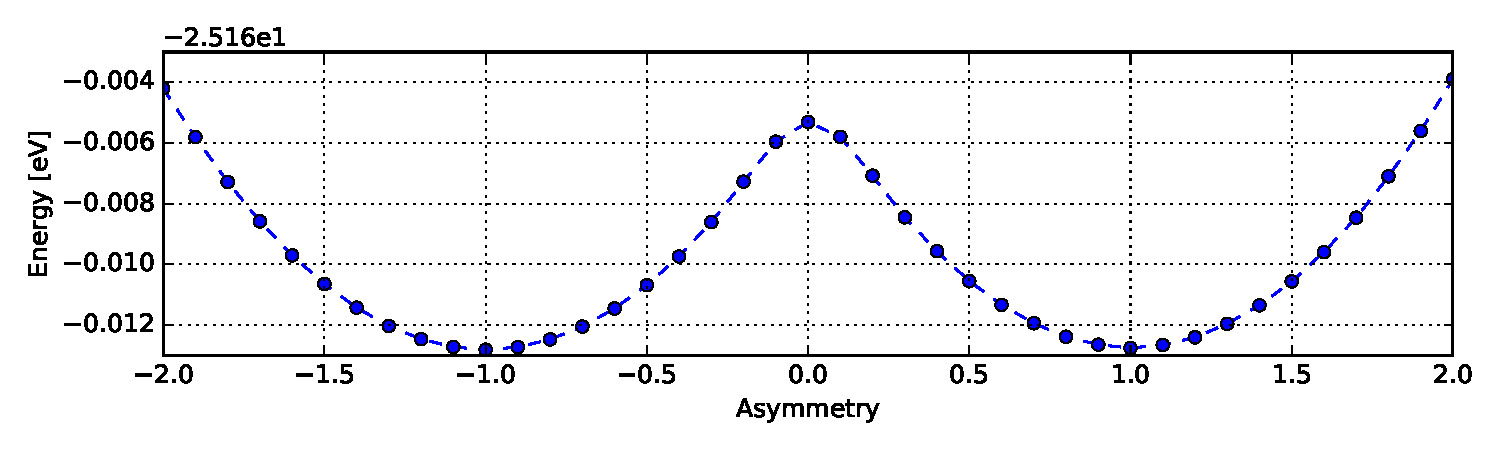
\includegraphics[width = \textwidth]{Images/polyacetylene/convergence/Potential_with_asymmetry}
	\caption{Mit $k$-Punkt am \textsc{Brillouin}-Zonen-Rand.}
	\label{image_potential_with_asymmetry}
	\end{subfigure}
	\begin{subfigure}{.85\textwidth}
	\centering
	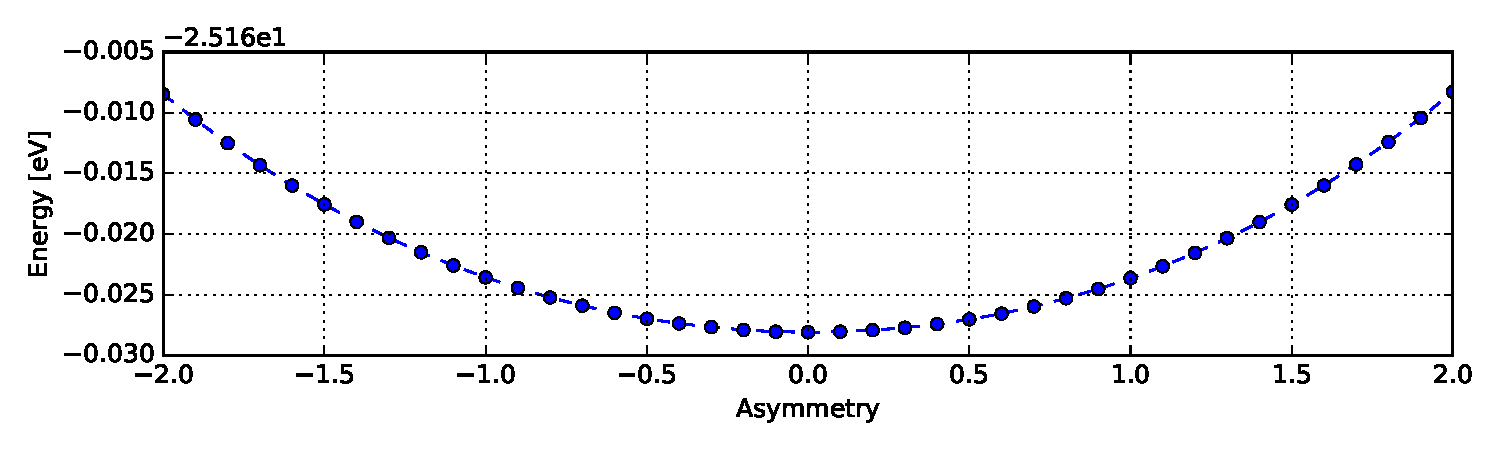
\includegraphics[width = \textwidth]{Images/polyacetylene/convergence/Potential_without_asymmetry}
	\caption{Ohne $k$-Punkt am \textsc{Brillouin}-Zonen-Rand.}
	\label{image_potential_without_asymmetry}
	\end{subfigure}
	\caption{Grundzustandsenergie in Abhängigkeit von der Asymmetrie $\nicefrac{u}{u_0}$.}
\end{figure}
\end{frame}

\begin{frame}
\begin{figure}
\centering
\begin{tikzpicture}[show background rectangle, scale = .65]
	\foreach \x in {0,...,7}{
		\draw[line width=1pt] (\x,0) .. controls (\x + 1, 2) and (\x - 1 , 2) .. cycle .. controls (\x + 1, -2) and (\x - 1 , -2) .. cycle;
	}
	\foreach \x in {0, 4}
	\foreach \y in {0, 1}
	\foreach \z in {-1, 1}
	\node at (\x + \y - \z + 1, \z) {\large +};
	\foreach \x in {0, 4}{
		\foreach \y in {0, 1}{
			\foreach \z in {-1, 1}{
				\node at (\x + \y - \z + 1, -\z) {\large -};
	}}}
	\draw[line width = 0.2] (-0.1, -1.8) -- +(-0.3, 0) -- +(-0.3 ,3.6) -- +(0,3.6);
	\draw[line width = 0.2] (1.1, -1.8) -- +(0.3, 0) -- +(0.3 ,3.6) -- +(0,3.6);
	\draw[line width = 0.2] (3.9, -1.8) -- +(-0.3, 0) -- +(-0.3 ,3.6) -- +(0,3.6);
	\draw[line width = 0.2] (7.1, -1.8) -- +(0.3, 0) -- +(0.3 ,3.6) -- +(0,3.6);
	\draw[dotted, line width = 1.5] (-0.6,0) -- (-1,0);
	\draw[dotted, line width = 1.5] (7.6,0) -- (8,0);
\end{tikzpicture}
\caption{Schema: p-Orbitale von alternierender $\pi$-Bindung.}
\end{figure}
\begin{figure}[]
	\centering
	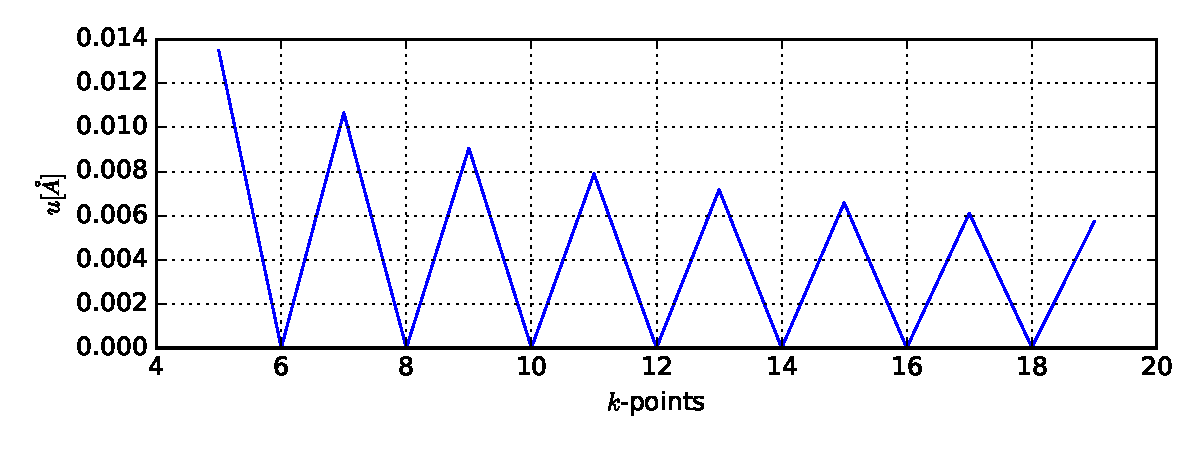
\includegraphics[width = .7\textwidth]{Images/polyacetylene/convergence/displacement_double_cell_poly}
	\caption{Verschiebung $u$ in Abhängigkeit von den $k$-Punkten für eine Einheitszelle mit vier CH-Gruppen.}
	\label{image_disp_double_cell_poly}
\end{figure}
\end{frame}

\begin{frame}
\begin{figure}
	\centering
	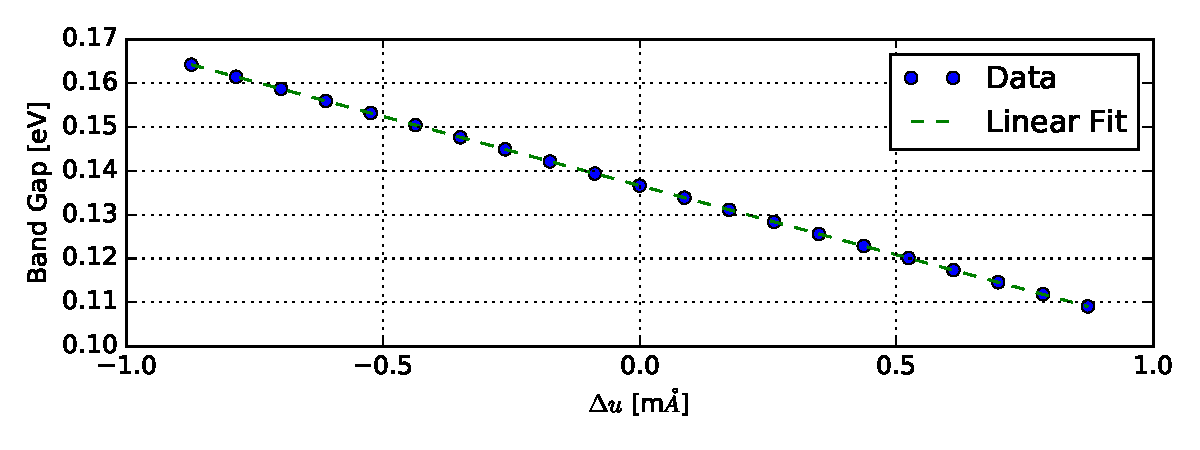
\includegraphics[width = 9cm]{Images/polyacetylene/bands/alpha}
	\caption{Bandlücke in Abhängigkeit von der Verschiebung.}
	\label{image_alpha_fit}
\end{figure}
\end{frame}

\begin{frame}
\begin{figure}
\centering
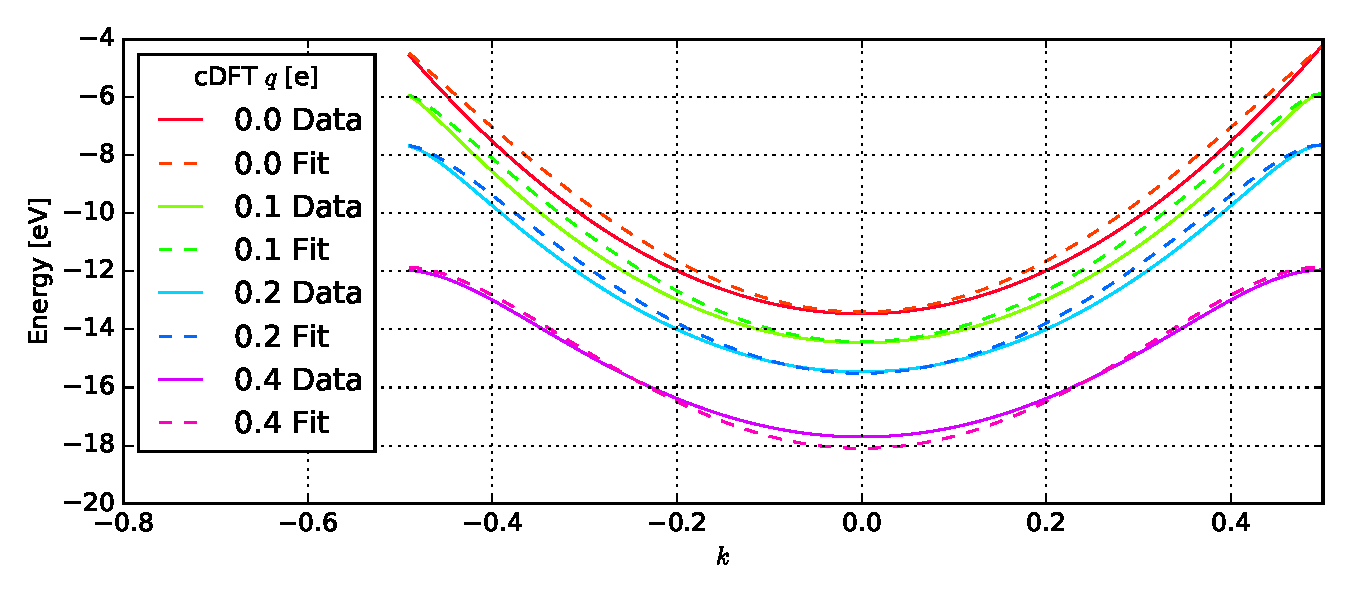
\includegraphics[width = 8cm]{Images/Hydrogen/charging/3D_cuts}
\caption{Wasserstoff-Kette}
\label{image_hydrogen_3D_slices}
\end{figure}
\vspace*{-.7cm}
\begin{figure}
\centering
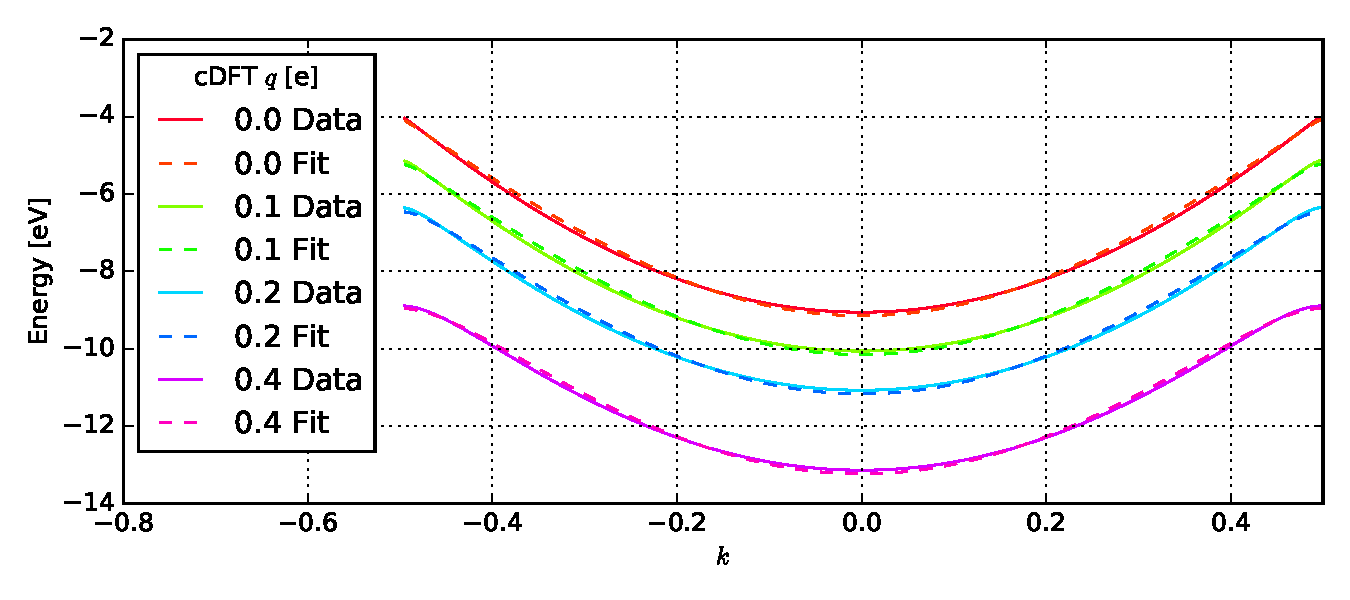
\includegraphics[width = 8cm]{Images/polyacetylene/charging/3D_cuts}
\caption{\emph{trans}-Polyacetylen}
\end{figure}
\end{frame}

\begin{frame}
\begin{figure}
	\centering
	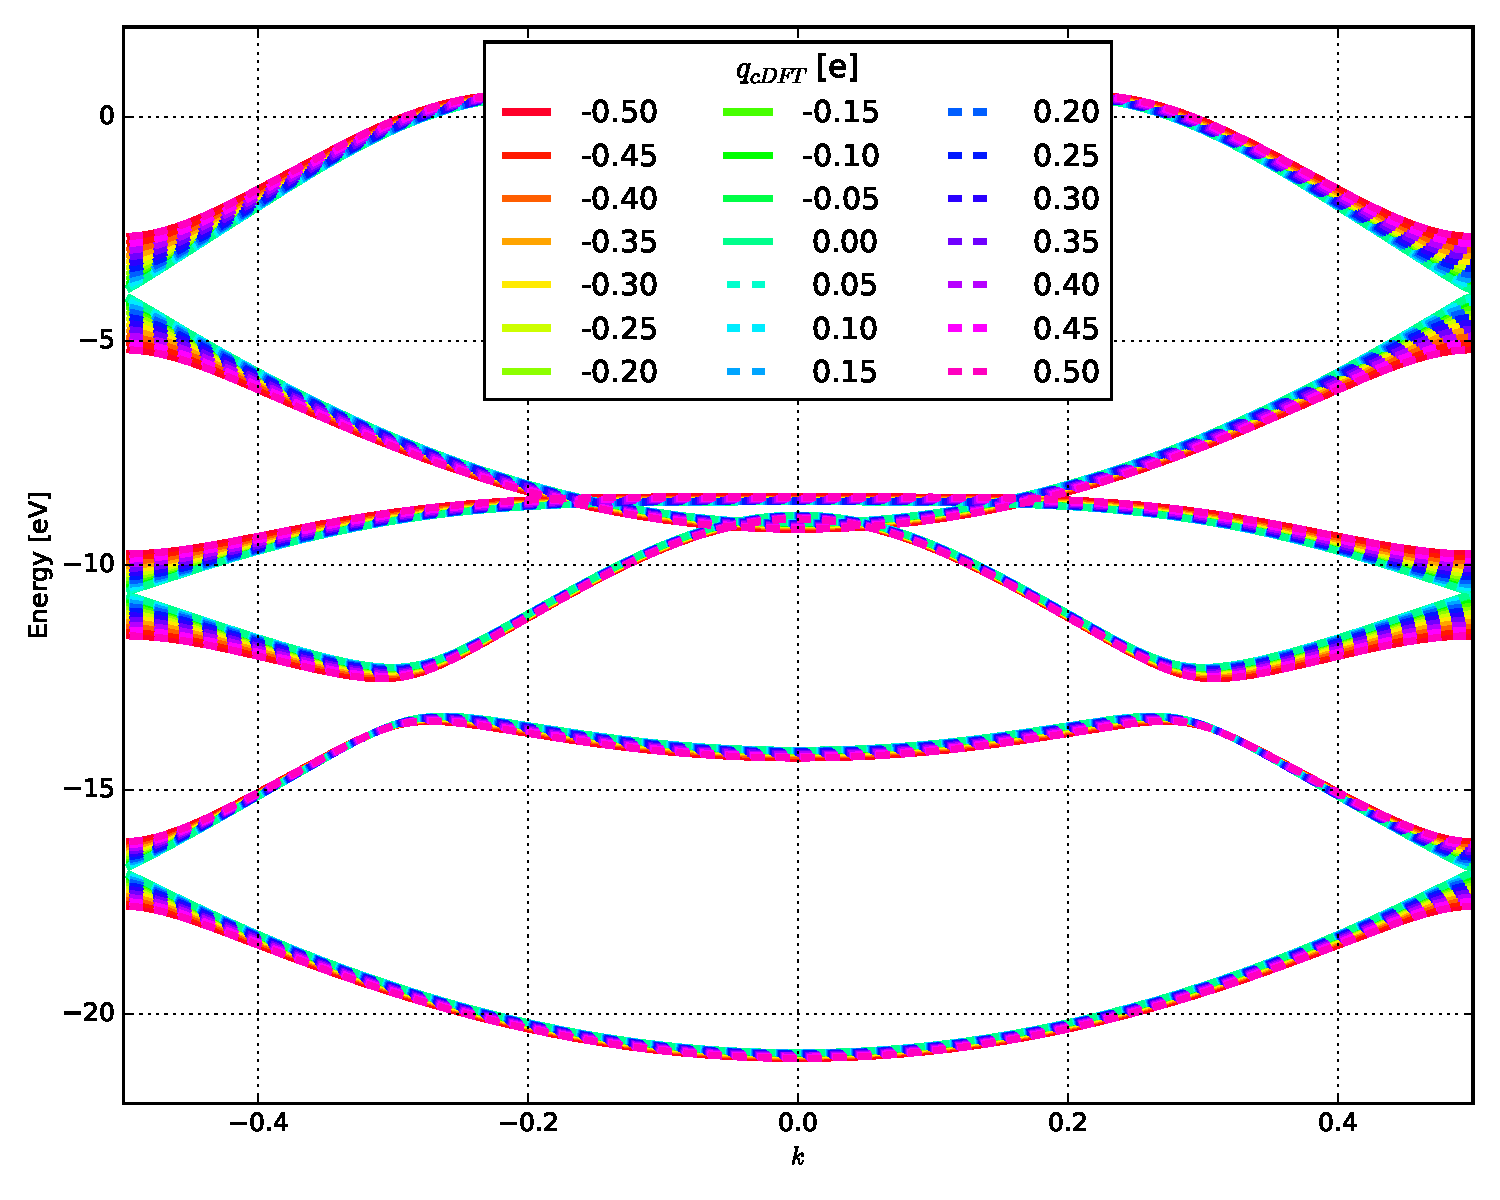
\includegraphics[width = 9.5cm]{Images/polyacetylene/charging/band_structure_q_1}
	\caption{Bandstruktur von \emph{trans}-Polyacetylen für verschiedene Ladungsverschiebungen.}
	\label{image_polyacetylene_band_structure_charging}
\end{figure}
\end{frame}

\begin{frame}
\begin{figure}
	\centering
	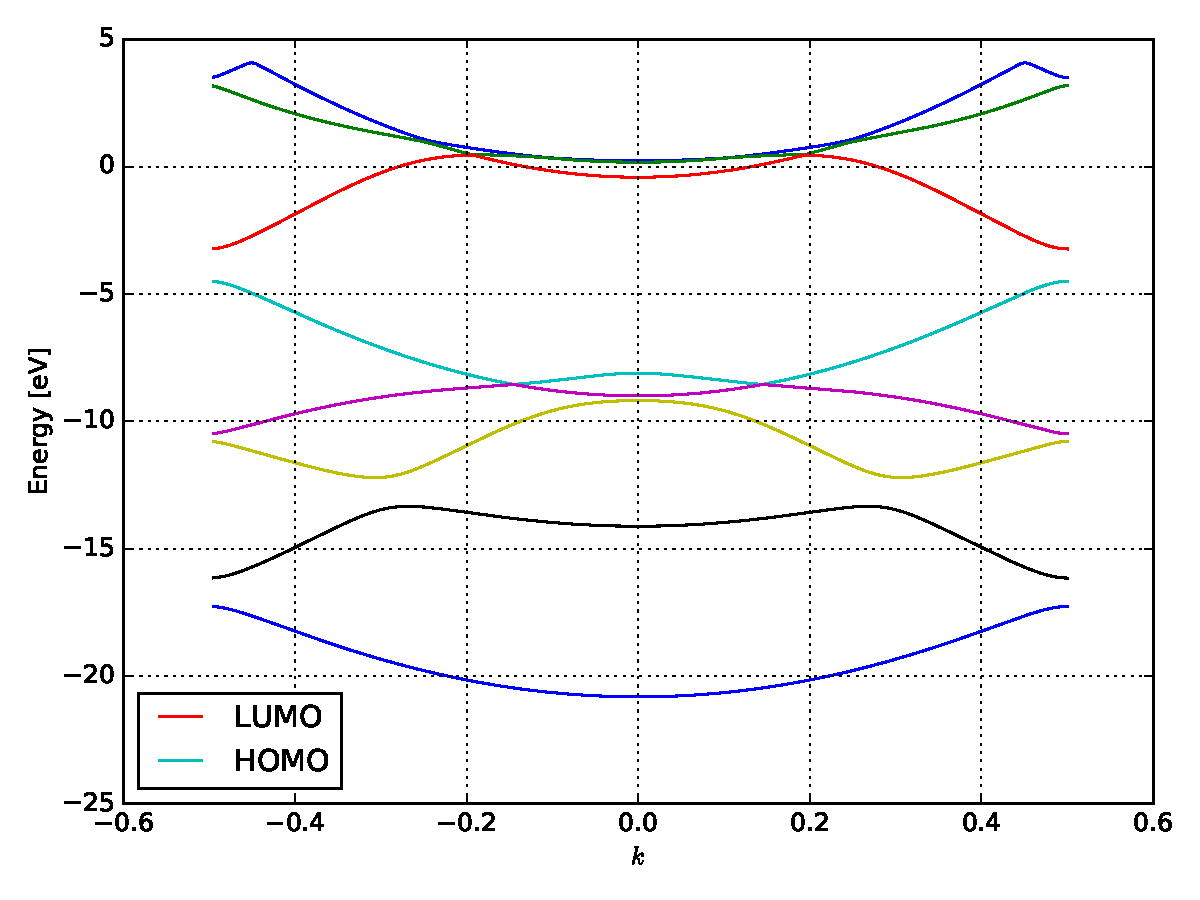
\includegraphics[width = 10cm]{Images/polyacetylene/bands/bandstructure_manually_displaced}
	\caption{Bandstruktur von \emph{trans}-Polyacetylen für $u = \unit[0.042]{\AA}$}
	\label{image_manually_displaced_poly_bandstructure}
\end{figure}
\end{frame}